\documentclass[dvipdfmx,titlepage,a4j]{jsarticle}

\usepackage{url}
\usepackage{graphicx}
\usepackage{listings,jvlisting}
\usepackage{amsmath,amssymb}
\usepackage{graphicx}
\usepackage[yen]{okuverb}
\usepackage{ascmac}
\usepackage{fancybox}
\usepackage{fancyvrb}
\usepackage{fancyhdr}
\usepackage{lastpage}
\usepackage{caption}
\usepackage{subcaption}
\usepackage{here}

\fancypagestyle{foot}
{
\fancyhead[C]{}
\fancyfoot[C]{\thepage / \pageref{LastPage}}
\renewcommand\headrulewidth{0.4pt}
}

%ここからソースコードの表示に関する設定
\lstset{
  language={C++},
  basicstyle={\ttfamily},
  identifierstyle={\small},
  commentstyle={\smallitshape},
  keywordstyle={\small\bfseries},
  ndkeywordstyle={\small},
  stringstyle={\small\ttfamily},
  frame={tb},
  tabsize={2},
  breaklines=true,
  columns=[l]{fullflexible},
  numbers=left,
  xrightmargin=0zw,
  xleftmargin=3zw,
  numberstyle={\scriptsize},
  stepnumber=1,
  numbersep=1zw,
  lineskip=-0.5ex
}

\title{タイトル}
\author{waarrk}
\date{2023年2月1日}

\begin{document}

\begin{titlepage}
    \centering
    \vspace*{2cm}

    \vspace{1cm}

    {\LARGE \textbf{つぼとボールのシミュレーション}}

    \vspace{0.5cm}

    {\LARGE 2024年度開講 認識工学レポート}

    \vspace{1.5cm}

    {\textbf{千葉工業大学 先進工学部 未来ロボティクス学科}\\}
    {\textbf{22C1704 鷲尾 優作}}

    \vfill

    {\large 2024年7月23日}

    \vspace{1cm}
\end{titlepage}

\section{目的}
本稿では、隠れマルコフモデルの代表的な問題である、つぼとボールのモデルをシミュレーションし、その動作を確認することで、隠れマルコフモデルの理解を深める.

\section{シミュレーション}

以下のステップでシミュレーションを行い、隠れマルコフモデルの動作を確認する.

\begin{enumerate}
    \item 初期状態からシミュレーションを開始し、状態遷移と観測を繰り返す
    \item 各状態の滞在時間と観測の出現回数を定量的に評価する
    \item 状態ごとの観測確率を計算し、設定されたモデルの確率と一致するかを確認する
\end{enumerate}

\subsection{問題設定}

つぼとボールのモデル(urn and ball model)は、隠れマルコフモデル(Hidden Markov Model, HMM)の一例として用いられる.このモデルでは、複数のつぼ(urn)と、それぞれのつぼから取り出されるボールの色が観測される.以下に、具体的な問題設定を示す.

\paragraph{状態と観測}
\begin{itemize}
    \item \textbf{状態}: 各つぼの状態(Urn1, Urn2, Urn3)
    \item \textbf{観測}: つぼから取り出されるボールの色(Red, Blue)
\end{itemize}

\paragraph{初期確率分布}

システムが開始する初期状態の確率分布を以下のように設定する.

\[
    \begin{array}{ccc}
        \text{Urn1} & \text{Urn2} & \text{Urn3} \\
        0.6         & 0.3         & 0.1         \\
    \end{array}
\]

\paragraph{状態遷移確率}

各状態から他の状態への遷移確率を以下のように設定する.

\[
    \text{状態遷移確率} =
    \begin{bmatrix}
        0.7 & 0.2 & 0.1 \\
        0.3 & 0.5 & 0.2 \\
        0.2 & 0.3 & 0.5
    \end{bmatrix}
\]

\paragraph{観測確率}

各状態において特定の色のボールが取り出される確率を以下のように設定する.

\[
    \text{観測確率} =
    \begin{bmatrix}
        0.6 & 0.4 \\
        0.4 & 0.6 \\
        0.7 & 0.3
    \end{bmatrix}
\]

\subsection{評価方法}

シミュレーションの結果を以下の指標で定量的に評価する.

\begin{enumerate}
    \item \textbf{各状態の滞在回数}: 各つぼにどれくらい滞在していたかの回数を計算する
    \item \textbf{各観測の出現回数}: 各色のボールが何回出現したかを数える
    \item \textbf{状態ごとの観測確率}: 各状態にいるときに特定の色のボールがどれくらいの確率で出現したかを計算する
\end{enumerate}

\section{シミュレーション結果}

シミュレーションの結果を以下に示す.
図\ref{fig:sim}に、状態遷移と観測の変化をグラフ化して示す.

\begin{figure}[H]
    \centering
    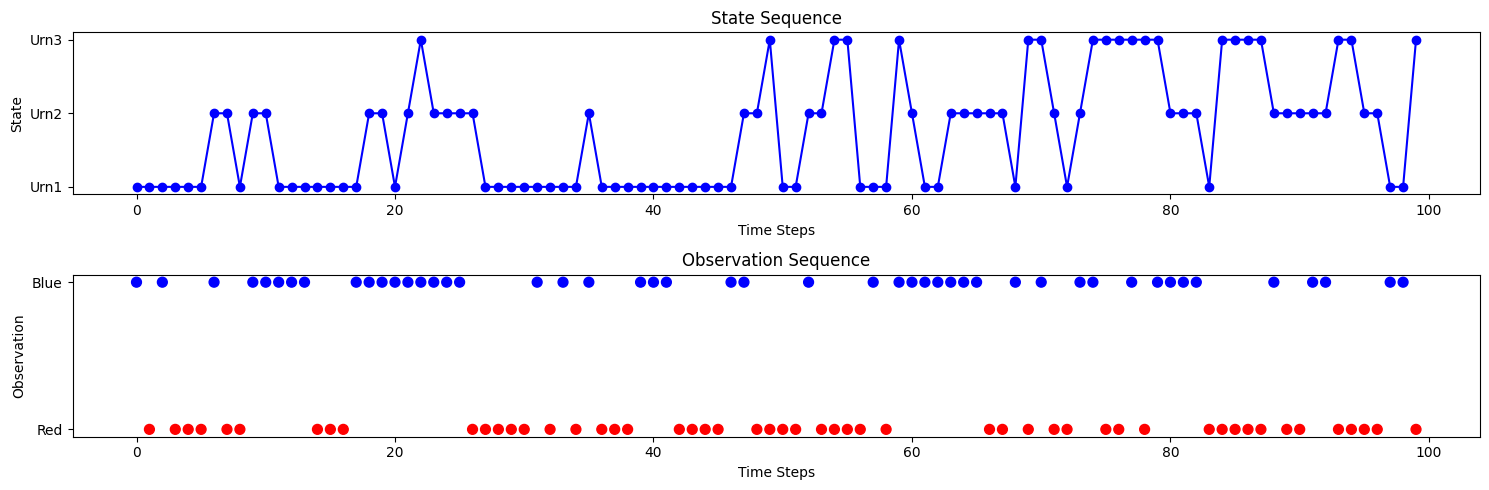
\includegraphics[width=1.0\textwidth]{picture/sim.png}
    \caption{シミュレーション結果}
    \label{fig:sim}
\end{figure}

\paragraph{状態の出現回数}
各状態の出現回数は以下の通りである.

\begin{itemize}
    \item Urn1 (State 0): 46回
    \item Urn2 (State 1): 34回
    \item Urn3 (State 2): 20回
\end{itemize}

\paragraph{観測の出現回数}
各観測の出現回数は以下の通りである.

\begin{itemize}
    \item Red (Observation 0): 52回
    \item Blue (Observation 1): 48回
\end{itemize}

\paragraph{状態ごとの観測確率}
各状態における観測確率は以下の通りである.

\begin{itemize}
    \item Urn1 (State 0):
          \begin{itemize}
              \item Red (Observation 0): 58.70\%
              \item Blue (Observation 1): 41.30\%
          \end{itemize}
    \item Urn2 (State 1):
          \begin{itemize}
              \item Red (Observation 0): 32.35\%
              \item Blue (Observation 1): 67.65\%
          \end{itemize}
    \item Urn3 (State 2):
          \begin{itemize}
              \item Red (Observation 0): 70.00\%
              \item Blue (Observation 1): 30.00\%
          \end{itemize}
\end{itemize}

\section{考察}

シミュレーション結果は、モデルの設定通りに動作していることを示している.以下に、各状態の出現回数や観測確率が設定通りであることを詳細に考察する

\subsection{各状態の出現回数について}

\begin{itemize}
    \item \textbf{Urn1 (State 0)}: 出現回数が46回と最も多い.初期確率が60\%であり、また自己遷移確率が70\%と高いため、長時間滞在することが多くなっている
    \item \textbf{Urn2 (State 1)}: 出現回数が34回であり、初期確率30\%および状態遷移確率のバランスから予想される範囲内である
    \item \textbf{Urn3 (State 2)}: 出現回数が20回と最も少ない.初期確率10\%および遷移確率が他の状態に比べて低いため、滞在時間が短くなっている
\end{itemize}

\subsection{各観測の出現回数について}

\begin{itemize}
    \item \textbf{Red (Observation 0)}: 出現回数が52回.各状態における観測確率に基づいて、全体の観測回数として合理的である
    \item \textbf{Blue (Observation 1)}: 出現回数が48回.Redの出現回数とほぼ均等であり、各状態の観測確率に基づいてバランスが取れている
\end{itemize}

\subsection{状態ごとの観測確率について}

\begin{itemize}
    \item \textbf{Urn1 (State 0)}:
          \begin{itemize}
              \item Red (Observation 0): 58.70\%であり、設定値の60\%に近い
              \item Blue (Observation 1): 41.30\%であり、設定値の40\%に近い
          \end{itemize}
    \item \textbf{Urn2 (State 1)}:
          \begin{itemize}
              \item Red (Observation 0): 32.35\%であり、設定値の40\%に近い
              \item Blue (Observation 1): 67.65\%であり、設定値の60\%に近い
          \end{itemize}
    \item \textbf{Urn3 (State 2)}:
          \begin{itemize}
              \item Red (Observation 0): 70.00\%であり、設定値の70\%に一致している
              \item Blue (Observation 1): 30.00\%であり、設定値の30\%に一致している
          \end{itemize}
\end{itemize}

\subsection{シミュレーションの精度と妥当性}

シミュレーションの結果は、モデルの設定に基づいた確率に沿っており妥当性があると判断できる.
また、設定された初期確率、状態遷移確率、および観測確率が合理的であり、モデルの妥当性が確認できる.シミュレーション回数を増やすことで、さらに結果の精度を高めることが可能である.

\section{付録}
\subsection{シミュレーションプログラム}

\lstinputlisting[caption=sim.png,label=prog:sim]{program/sim.py}

\nocite{*}
\bibliographystyle{jplain}
\bibliography{refs}

\end{document}
